\subsection{Opgave 16}

En cirkel $C$ og en linje $l$ er bestemt ved ligningerne
\begin{align*}
    C&:(x-4)^2 + (y-5)^2 = 3^2\\
    l&:y = x-2
\end{align*}
 a) Tegn cirklen og linjen i samme koordinatsystem.\\

 \ans
 Vi starter med at aflæse cirklens centrumskoordinat og cirklens radius. Vi ved at cirklens generelle ligning er givet ved
 \begin{align*}
     (x-a)^2 + (y-b)^2 = r^2
 \end{align*}
 Her er $C(a,b)$ cirklens centrumskoordinat og r er cirklens radius. Hvis vi bruger dette kan vi aflæse centrumskoordinatet til $C(4,5)$ og radius til $r = 3$. Vi kan nu indtegne cirklen i et koordinatsystem\\\\
 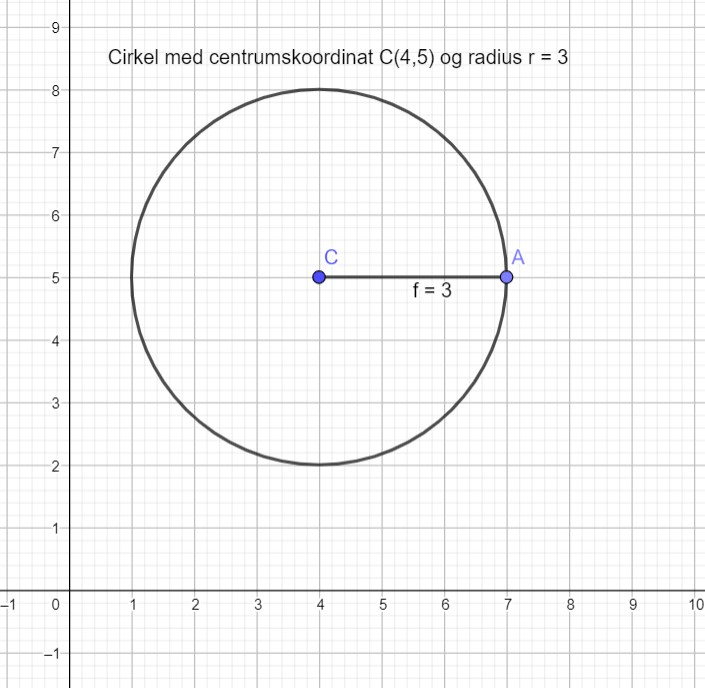
\includegraphics[width=8cm]{Opgave_11-20/Opgave_16/16.jpg}\\\\
 
 For at indtegne linjen skal vi aflæse linjens hældning, a og linjens skærings med y-aksen, b. Vi ved at en ret linje har den generelle form
 \begin{align*}
     y = ax+b
 \end{align*}
 Aflæser vi nu den givne linje får vi hældningen $a = 1$ og skæringen med y-aksen $b = -2$. Ud fra disse oplysninger kan vi nu indtegne vores linje i koordinatsystemet\\\\
 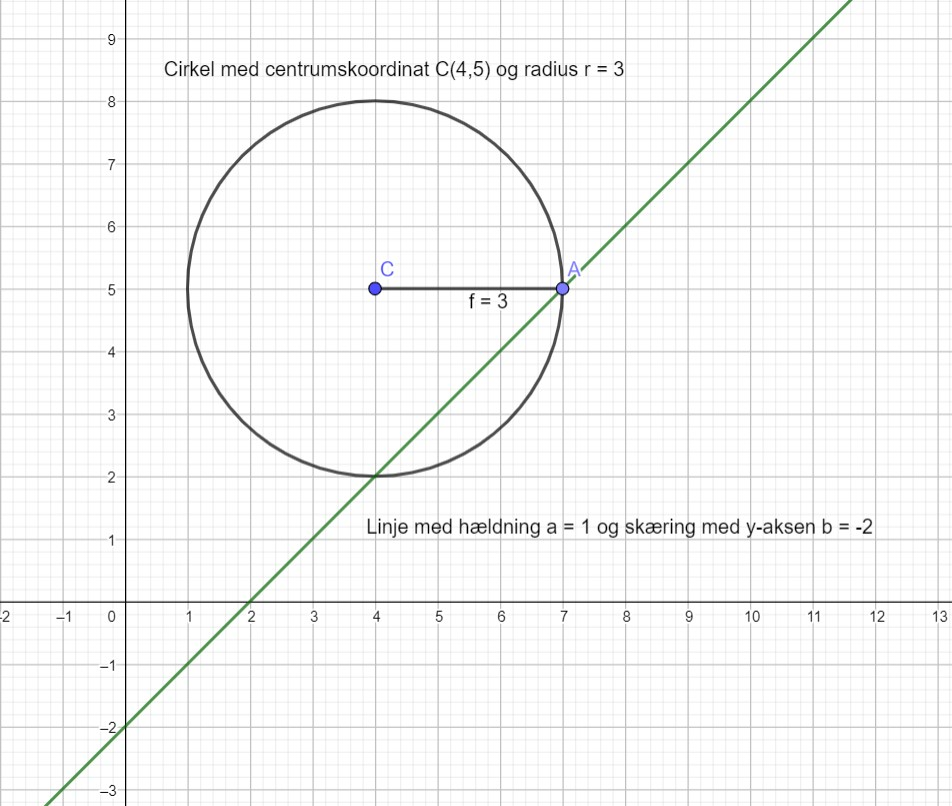
\includegraphics[width = 8cm]{Opgave_11-20/Opgave_16/16.1.jpg}\\\\
 
 b) Bestem skæringspunkterne mellem cirklen og linjen\\\\

 \ans
 
 Ud fra koordinatsystemet i opgave 16a kan vi se at cirklen og linjen skærer hinanden i 2 punkter. For at bestemme disse skæringspunkter sætter vi linjens ligning $y = x-2$ ind på y's plads i cirklens ligning
 \begin{align*}
     &(x-4)^2 + (x-2-5)^2 = 3^2\\
     \; \Updownarrow &\\
     &(x-4)^2 + (x-7)^2 = 9\\
 \end{align*}
 Vi beregner nu de 2 parenteser ved at bruge reglen $(a-b)^2 = a^2+2\cdot a\cdot (-b) + (-b)^2$
 \begin{align*}
     (x-4)^2 = x^2 +2\cdot x \cdot (-4) + (-4)^2 = x^2 -8x + 16\\
     (x-7)^2 = x^2 +2\cdot x \cdot (-7) + (-7)^2 = x^2 -14x + 49
 \end{align*}
 Indsætter vi dette får vi nu
 \begin{align*}
    &(x-4)^2 + (x-7)^2 = 9\\
    \; \Updownarrow &\\ 
    &x^2-8x+16+x^2-14x+49 = 9\\
    \; \Updownarrow &\\
    &x^2+x^2 -8x - 14x + 16+49=9\\
    \; \Updownarrow &\\
    &2x^2 - 22x + 65 = 9
 \end{align*}
 Vi trækker nu 9 fra på begge sider 
 \begin{align*}
     &2x^2 -22x +65-9 = 9-9\\
     \; \Updownarrow &\\
     &2x^2 -22x 56 = 0
 \end{align*}
 Nu findes vi løsningerne til det ovenstående andengradsligning ved først at beregne determinanten 
 \begin{align*}
     d = b^2 -4ac = (-22)^2 -4\cdot 2\cdot 56 = 36
 \end{align*}
 Nu bestemmer vi løsningerne altså x-koordinatet til skæringen mellem cirklen og linjen
 \begin{align*}
     x_1 = \frac{-b+\sqrt{d}}{2a}=\frac{22+\sqrt{36}}{2\cdot 2}=\frac{22+6}{4}=\frac{28}{4}=7\\
     x_2 = \frac{-b-\sqrt{d}}{2a}=\frac{22-\sqrt{36}}{2\cdot 2}=\frac{22-6}{4}=\frac{16}{4} = 4
 \end{align*}
 For at finde de tilsvarende skæringer med y-aksen indsætter vi de fundne x-værdier i linjens ligning
 \begin{align*}
     y_1 = x_1 -2 = 7-2 = 5\\
     y-2 = x_2 -2 = 4-2 = 2
 \end{align*}
 Vi har altså føgende skæringspunkter mellem linjen og cirklen
 \begin{align*}
     S_1=(x_1, y_1)=(7,5)\\
     S_2 =(x_2,y_2)=(4,2)
 \end{align*}
 Hvis vi sammenligner med tegningen vi får fra opgave 16a kan vi se at skærngspunkterne stemmer.